\addtocontents{toc}{\protect\setcounter{tocdepth}{2}}
\begin{appendices}
\renewcommand\thefigure{S\arabic{figure}} % modify \thefigure, *not* \figurename
\newcounter{myfig} 

\renewcommand\thetable{S\arabic{table}} % modify \thefigure, *not* \figurename
\newcounter{mytable} 
    
\etocsetnexttocdepth{3}
\etocsettocstyle{\section*{Extended Data and Supplementary Information}}{}
\cftsubsubsecindent 0pt
\tableofcontents


\clearpage


\section{Satute applied to simulated data}
\subsection{Branch length estimates}

\iffalse
\begin{figure}[H]
    \centering
    \includegraphics[scale=0.5]{branch-length-estimates-true-tree-A8+B8-JC-min4percent_1000bp.pdf}
    \vspace{0.25cm}
    \caption{\textbf{Branch length estimates of the simulations for the 16-taxon tree in the  true-tree topology with ML-estimated branch lengths scenario ({\color{truetreeML} dark red}).} The figure shows all $1000$ ML-estimated branch lengths for each branch length parameter of the considered branch
$AB$ of simulation tree  as box plots. The solid line represents the identity function.}
    \label{suppfig:branchlengths_scenario2}
\end{figure}

\noindent\textbf{Protocol for Supplementary Fig.\,\ref{suppfig:branchlengths_scenario2}:} This protocol follows the Protocol for Fig.\,\ref{fig:simulation}b, see Methods \ref{sec:protocol_simulation_16taxa}. For the second scenario (true-tree topology with ML-estimated branch lengths, {\color{truetreeML} dark red}), we additionally extracted the  ML-estimated branch lengths for each alignment of length $1000$bp. The $1000$ ML-estimated branch lengths for each branch length parameter of
$AB$ in the simulation tree are presented as box plots. 
\fi

\begin{figure}[H]
    \centering
    \includegraphics[scale=0.5]{branch-length-estimates-ML-tree-A8+B8-JC-min4percent_1000bp.pdf}
    \vspace{0.25cm}
    \caption{\textbf{Branch length estimates of the simulations for the 16-taxon tree in the  ML-tree scenario ({\color{MLtree} light green}).} The figure shows the branch length estimates of the inferred ML-trees that contain a branch splitting the taxa of $\mathbb{T}_A$ and $\mathbb{T}_B$.  These estimates, for each branch length parameter of the considered branch $AB$ in the simulation tree, are presented as box plots. The solid line represents the identity function.}
    \label{suppfig:branchlengths_scenario3}
\end{figure}
\noindent\textbf{Protocol for Supplementary Fig.\,\ref{suppfig:branchlengths_scenario3}:} This protocol follows the protocol described for Fig.\,\ref{fig:simulation}b, see Methods \ref{sec:protocol_simulation_16taxa}. For third scenario (ML-tree, {\color{MLtree} light green}), we additionally extracted the branch length estimates of the inferred ML-trees for each alignment of length $1000$bp, provided the ML-tree contains a branch that splits the taxa of $\mathbb{T}_A$ and $\mathbb{T}_B$. The  branch lengths estimates (up to $1000$) for each branch length parameter of $AB$ in the simulation tree are presented as box plots.
\bigskip

\subsection{Effect of short branches}
% currently Fig S2 (A8-B8, min blen 1/seqlen)
\begin{figure}[H]
    \centering
    
\includegraphics[scale=0.5]{supplementary_figure_effect_short_branches.pdf}
    \vspace{0.25cm}
           \caption{\textbf{Effect of short branches on the test for phylogenetic information.}
          Fraction of informative instances when testing the depicted branch in various scenarios: the true-tree ({\color{truetree} pink}), the true-tree topology with ML-estimated branch lengths ({\color{truetreeML} violet}), the inferred ML-tree including branch lengths ({\color{MLtree} blue}), and the inferred ML-tree including branch lengths with Bonferroni-corrected test ({\color{MLtreeBonferroni} green}). The analysis was performed in an external branch of a 5-taxon tree (\textbf{a}) and the central branch of a balanced 16-taxon tree (\textbf{b}). Dashed, solid, and alternating dashed lines represent the results for $100$, $1000$, and $10000$ sites, respectively. If many of the branch lengths of the tree are close to zero, then the test with Bonferroni correction becomes conservative and the rejection level falls below $5\%$ ({\color{MLtreeBonferroni}green}).}
	\label{suppfig:simulation_shortBranches}
\end{figure}


\textbf{Protocol for Supplementary Fig.\,\ref{suppfig:simulation_shortBranches}:} We closely followed the Protocol for Fig.\,\ref{fig:simulation}b, see Methods \ref{sec:protocol_simulation_16taxa}. The only difference was that,  the internal and external branch lengths was drawn from the distributions (Fig.\,\ref{suppfig:EvoNAPS_branch_distribution}) of all internal and external branch lengths, respectively, as stored in the EvoNAPS database \citepSupp[\url{http://evonaps.cibiv.univie.ac.at}]{reden2023} for the sources OrthoMaM, Lanfear and TreeBase with a lower minimum length of $1/n$ (instead of $0.04$), where $n$ is the  alignment length.

\begin{figure}[H]
    \centering
    
\includegraphics[scale=0.5]{EvoNAPS_branch_length_distribution.pdf}
    \vspace{0.25cm}
    \caption{\textbf{Empirical branch length distribution from EvoNAPS:} The figure shows the distributions of all internal and external branch lengths, respectively, as stored in the EvoNAPS database for the sources OrthoMaM, Lanfear and TreeBase.}
    \label{suppfig:EvoNAPS_branch_distribution}
\end{figure}

\medskip

%%% Tab. Bootstrap values %%%
\subsection{Bootstrap support values}
\begin{table}[hb]
    \centering
    \begin{tabular}{|c|r|r|r|r|}
\hline
Simulation branch & $AB$ split & Average  & Minimum & Informative\\
length of $AB$& contained   & BS value & BS value & instances (\%) \\
\hline
0.1 &  993 &  93.32 &  14 & 100   \\
0.2 &  999 &  99.19 &  74 & 100  \\
0.3 & 1000 &  99.86 &  87 & 100   \\
0.4 & 1000 &  99.95 &  93 & 100 \\
0.5 & 1000 &  99.99 &  97 & 100   \\
0.8 & 1000 & 100  & 100 &  99.1 \\
1   & 1000 & 100  & 100 &  92.4 \\
1.5 & 1000 & 100  & 100 &  49.7 \\
2   & 1000 & 100  & 100 &  21.6 \\
2.5 & 1000 & 100  & 100 &   9.6 \\
3   & 1000 & 100  & 100 &   5.9 \\
3.5 & 1000 & 100  & 100 &   4.3 \\
4   & 1000 & 100  & 100 &   4.6 \\
5   & 1000 & 100  & 100 &   3.8 \\
7.5 & 1000 & 100  & 100 &   3.5 \\
10  & 1000 & 100  & 100 &   4.3 \\
\hline
    \end{tabular}
    \vspace{0.25cm}
    \caption{
        \textbf{Bootstrap support (BS) values of the simulations for the 16-taxon tree.} For each branch length of $AB$ in the simulation tree as shown in Fig.\,\ref{fig:simulation}b, $1000$ DNA alignments with sequence length of $100$bp were simulated under JC model. For each alignment, we conducted a bootstrap analysis with 100 replicates. The table summarizes the number of inferred ML-trees containing a branch that splits the taxa of $\mathbb{T}_A$ and $\mathbb{T}_B$ ($AB$ split contained), along with the average  and minimum bootstrap support values over all $1000$ analyses.  For comparison, we include the fraction of informative instances of Fig.\,\ref{fig:simulation}b for an alignment length of $100$ sites in the scenario ML-tree with corrected test (dashed line, {\color{MLtreeBonferroni} green}). 
    }
    \label{supptab:bootstrap}
    \end{table}

\noindent\textbf{Protocol for Table\,\ref{supptab:bootstrap}:} This protocol partially follows the one described for Fig.\,\ref{fig:simulation}b, see Methods \ref{sec:protocol_simulation_16taxa}.

\medskip

The considered simulation tree is the 16-taxon tree shown in Fig.\,\ref{fig:simulation}b. Our focus is on the internal branch $AB$, connecting the root $A$ of a balanced $8$-taxon subtree $\mathbb{T}_A$ was connected to the root $B$ of a balanced $8$-taxon subtree $\mathbb{T}_B$. All branch lengths in $\mathbb{T}_A$ and $\mathbb{T_B}$ were drawn between $0.04$ and $0.2$ from the distributions (see Supplementary Fig.\,\ref{suppfig:EvoNAPS_branch_distribution}) of all internal and external branch lengths, respectively, as stored in the EvoNAPS database \citepMeth[\url{http://evonaps.cibiv.univie.ac.at}]{reden2023} for the sources OrthoMaM, Lanfear and TreeBase. While the branch length of $AB$ varied among $\{0.1, 0.2, 0.3, 0.4, 0.5, 0.8, 1.0, 1.5, 2.0, 2.5, 3.0, 3.5, 4.0, 5.0, 7.5, 10.0\}$. For each parameterization, we simulated sets of $1000$ DNA alignments with sequence length of $100$ sites using Seq-Gen \citepMeth[v1.3.4;][]{Rambaut1997} under the JC model. For each alignment, we conducted a bootstrap analysis with $100$ replicates using IQ-Tree \citepMeth[2.2.2.7;][]{minh2020}. For each of the $1000$ considered ML-tree, we determined if a branch exists that splits the taxa of $\mathbb{T}_A$ and $\mathbb{T}_B$ (i.e., $AB$ split contained). For the ML-trees containing this split, the bootstrap support value of branch $AB$ was computed using $100$ resamplings, allowing us to calculate the average and minimum BS values.

\medskip


For comparison, we include the fraction of informative instances of Fig.\,\ref{fig:simulation}b for an alignment length of $100$bp in the ML-tree \& Bonferroni correction scenario (dashed line, {\color{MLtreeBonferroni} green}). See  Protocol for Fig.\,\ref{fig:simulation}b (Methods \ref{sec:protocol_simulation_16taxa}).

\medskip

The cases of alignment lengths $n=1000$ and $n=10000$ sites are not represented because, for all simulation branch lengths of $AB$, the $1000$ ML-trees consistently contained the $AB$ split, and the branch $AB$ had a minimum BS value of $100$.

\medskip


\subsection{Placement of the reconstructed branch in the ML-tree}


\begin{table}[hb]
    \centering
    \begin{tabular}{|r|c|r|r|r|}
\hline
 &  &\multicolumn{3}{c|}{Reconstructed branch $AB$}\\
Alignment &Simulation branch&   Connecting  & Connecting &  Connecting\\
length &length of $AB$ &     2 external & 1 external +  & 2 internal \\
&&     branches & 1 internal branch & branches\\
\hline
100	&0.1	&  0	& 10 & 990 \\
100	&0.2	&  1	& 44 & 955 \\
100	&0.3	&  4	& 65 & 931 \\
100	&0.4	& 10	&120 & 870 \\
100	&0.5	& 29	&201 & 770 \\
100	&0.8	&146	&464 & 390 \\
100	&1   	&317	&442 & 241 \\
100	&1.5	&601	&323  & 76 \\
100	&2  	&736	&238  & 26 \\
100	&2.5	&799	&190 &  11 \\
100	&3  	&783	&206 &  11 \\
100	&3.5	&812	&179 &   9 \\
100	&4      &836	&159 &   5 \\
100	&5  	&834	&160 &   6 \\
100	&7.5	&844	&145 &  11 \\
100	&10 	&828	&162 &  10 \\
\hline
    \end{tabular}
    \vspace{0.25cm}
    \caption{
        \textbf{Placement of the reconstructed branch $AB$ in the ML-tree for the 16-taxon tree.}
        For each parameterization of the 16-taxon tree, we simulated sets of $1000$ DNA alignments with a sequence length of $100$ sites under the JC model. For each alignment, the ML-tree was inferred under the JC model. All ML-trees included a branch that splits the taxa of $\mathbb{T}_A$ and $\mathbb{T}_B$. By examining the splits of the trees, we determined how many $AB$ branches connect either two external branches of the subtrees $\mathbb{T}_A$ and $\mathbb{T}_B$, one external to one internal branch, or two internal branches.
   }
    \label{supptab:bonferroni_correction}
    \end{table}\hfill\\

\begin{table}[hb]
    \centering
    \begin{tabular}{|r|c|r|r|r|}
\hline
 &  &\multicolumn{3}{c|}{Reconstructed branch $AB$}\\
Alignment &Simulation branch&   Connecting  & Connecting &  Connecting\\
length &length of $AB$ &     2 external & 1 external +  & 2 internal \\
&&     branches & 1 internal branch & branches\\
\hline
1000	&0.1	&  0	& 0  & 1000 \\
1000	&0.2	&  0	& 0  & 1000 \\
1000	&0.3	&  0	& 0  & 1000 \\
1000	&0.4	&  0	& 0  & 1000 \\
1000	&0.5	&  0	& 0  & 1000 \\
1000	&0.8	&  0   	& 0  & 1000 \\
1000	&1   	& 0	    & 9  & 991 \\
1000	&1.5	&50	    &266 & 684 \\
1000	&2  	&386	&427 &187 \\
1000	&2.5	&616	&330 &54 \\
1000	&3  	&697	&279 &24 \\
1000	&3.5	&752	&239 & 9 \\
1000	&4      &771	&219 &10\\
1000	&5  	&776	&211 &13 \\
1000	&7.5	&776	&216 &8 \\
1000	&10 	&809	&182 &9 \\
\hline
    \end{tabular}
    \vspace{0.25cm}
    \caption{
        \textbf{Placement of the reconstructed branch $AB$ in the ML-tree for the 16-taxon tree.}
        For each parameterization of the 16-taxon tree, we simulated sets of $1000$ DNA alignments with a sequence length of $1000$ sites under the JC model. For each alignment, the ML-tree was inferred under the JC model. All ML-trees included a branch that splits the taxa of $\mathbb{T}_A$ and $\mathbb{T}_B$. By examining the splits of the trees, we determined how many $AB$ branches connect either two external branches of the subtrees $\mathbb{T}_A$ and $\mathbb{T}_B$, one external to one internal branch, or two internal branches.
   }
    \label{supptab:bonferroni_correction_1000}
    \end{table}\hfill\\

\begin{table}[hb]
    \centering
    \begin{tabular}{|r|c|r|r|r|}
\hline
      &  &\multicolumn{3}{c|}{Reconstructed branch $AB$}\\
Alignment &Simulation branch&   Connecting  & Connecting &  Connecting\\
length &length of $AB$ &     2 external & 1 external +  & 2 internal \\
&&     branches & 1 internal branch & branches\\
\hline
10000 &0.1	&  0	& 0  & 1000 \\
10000 &0.2	&  0	& 0  & 1000 \\
10000 &0.3	&  0	& 0  & 1000 \\
10000 &0.4	&  0	& 0  & 1000 \\
10000 &0.5	&  0	& 0  & 1000 \\
10000 &0.8	&  0   	& 0  & 1000 \\
10000 &1   	&  0   	& 0  & 1000 \\
10000 &1.5	& 0   	& 0  & 1000 \\
10000 &2  	& 1	    &22  &977 \\
10000 &2.5	&80	    &352 &568 \\
10000 &3  	&378	&475  &147 \\
10000 &3.5	&556	&399  &45 \\
10000 &4    &657	&317  &26\\
10000 &5  	&699	&291  &10 \\
10000 &7.5	&718	&274  & 8 \\
10000 &10 	&722	&270  & 8\\
\hline
    \end{tabular}
    \vspace{0.25cm}
    \caption{
        \textbf{Placement of the reconstructed branch $AB$ in the ML-tree for the 16-taxon tree.}
        For each parameterization of the 16-taxon tree, we simulated sets of $1000$ DNA alignments with a sequence length of $10000$ sites under the JC model. For each alignment, the ML-tree was inferred under the JC model. All ML-trees included a branch that splits the taxa of $\mathbb{T}_A$ and $\mathbb{T}_B$. By examining the splits of the trees, we determined how many $AB$ branches connect either two external branches of the subtrees $\mathbb{T}_A$ and $\mathbb{T}_B$, one external to one internal branch, or two internal branches.
   }
    \label{supptab:bonferroni_correction_10000}
    \end{table}\hfill\\
   
\noindent\textbf{Protocol for Table\,\ref{supptab:bonferroni_correction}-\,\ref{supptab:bonferroni_correction_10000}:} This protocol partially follows the one described for Fig.\,\ref{fig:simulation}b, see Methods \ref{sec:protocol_simulation_16taxa}.

\medskip

The considered simulation tree is the 16-taxon tree shown in Fig.\,\ref{fig:simulation}b. Our focus is on the internal branch $AB$, connecting the root $A$ of a balanced $8$-taxon subtree $\mathbb{T}_A$ was connected to the root $B$ of a balanced $8$-taxon subtree $\mathbb{T}_B$. All branch lengths in $\mathbb{T}_A$ and $\mathbb{T_B}$ were drawn between $0.04$ and $0.2$ from the distributions (see Supplementary Fig.\,\ref{suppfig:EvoNAPS_branch_distribution}) of all internal and external branch lengths, respectively, as stored in the EvoNAPS database \citepMeth[\url{http://evonaps.cibiv.univie.ac.at}]{reden2023} for the sources OrthoMaM, Lanfear and TreeBase. While the branch length of $AB$ varied among $\{0.1, 0.2, 0.3, 0.4, 0.5, 0.8, 1.0, 1.5, 2.0, 2.5, 3.0, 3.5, 4.0, 5.0, 7.5, 10.0\}$. For each parameterization, we simulated sets of $1000$ DNA alignments with sequence length of $100$, $1000$ and $10000$ sites using Seq-Gen \citepMeth[v1.3.4;][]{Rambaut1997} under the JC model. For each alignment, we conducted a bootstrap analysis with $100$ replicates using IQ-Tree \citepMeth[2.2.2.7;][]{minh2020}. 

For each of the $1000$ considered ML-tree, we determined if a branch exists that splits the taxa of $\mathbb{T}_A$ and $\mathbb{T}_B$ (i.e.,  contains the $AB$ split). In this simulation, all ML-trees contained the $AB$ split. {\color{olive}Using  TreeShredder}, we checked for the existence of a split that contains either (a) all taxa of subtree $\mathbb{T}_A$ plus one taxon of subtree $\mathbb{T}_B$ or (b) all taxa of subtree $\mathbb{T}_B$ plus one taxon of subtree $\mathbb{T}_A$. If both cases (a) and (b) are fulfilled, the branch $AB$ connects two external branches of the subtrees $\mathbb{T}_A$ and $\mathbb{T}_B$. If  either (a) or (b) is fulfilled, but not both, then  branch $AB$ connects an internal branch of one subtree with an external branch of the other subtree. Otherwise the branch $AB$ connects only internal branches of the subtrees $\mathbb{T}_A$ and $\mathbb{T}_B$.
\clearpage
    
\subsection{Model misspecification simulations}
%%% currently Fig S1. (model mis-specification) %%%
\begin{figure}[H]
        \centering
        
\includegraphics[width=\linewidth]{figure_simulated_data_misspecification.pdf}
             \caption{\textbf{Performance of Satute in presence of model misspecification.} The plot shows the fraction of informative instances when testing the depicted branch in absence of model misspecification (true-tree, {\color{truetreeNoMisspecification}gold}) and in various scenarios with model misspecification: true-tree ({\color{truetree}pink}), the true-tree topology with ML-estimated branch lengths ({\color{truetreeML}red}), and the inferred ML-tree including branch lengths with Bonferroni correction ({\color{MLtreeBonferroni} green}). In all cases the alignments were simulated with a GTR model, while reconstruction and testing under model misspecification was performed using the JC \textbf{(a,d)}, K2P \textbf{(b,e)} or F81 \textbf{(c,f)} models. The branches tested were \textbf{(a-c)} the external branch $AB$ of a $5$-taxon tree and \textbf{(d-f)} the central branch $AB$ of a balanced $16$-taxon tree. Dashed, solid and alternating dashed lines represent the results for alignments with $100, 1000$ and $10000$ number of sites, respectively. }
	\label{suppfig:simulation_misspec}
 \end{figure}

\medskip

%%%%% Fig S1a-c - model misspecification simulation A4-B1 %%%%%
\noindent\textbf{Protocol for Supplementary Fig.\,\ref{suppfig:simulation_misspec}a-c:}\label{subsec:misspec_5tree} This protocol mostly follows the protocol of Fig.\,\ref{fig:simulation}a, see Methods \ref{sec:protocol_simulation_5taxa}.

\medskip

\noindent The considered simulation tree is the five-taxon tree shown in Fig.\,\ref{fig:simulation}a. Our focus is on the external branch $AB$, connecting taxon $B$ to the root $A$ of a balanced four-taxon subtree $\mathbb{T}_A$. All branch lengths in $\mathbb{T}_A$ were set to 0.2, while the branch length of $AB$ varied among $\{0.1, 0.2, 0.3, 0.4, 0.5, 0.8, 1.0, 1.5, 2.0, 2.5, 3.0, 3.5, 4.0, 5.0, 7.5, 10.0\}$. For each parameterization, we simulated sets of $1000$ DNA alignments with sequence length ${n = 100, 1000, 10000}$ sites using Seq-Gen \citepMeth[v1.3.4;][]{Rambaut1997} under a GTR model with rates $AC=0.6676$, $AG=3.7807$, $AT=4.2833$, $CG=0.5354$, $CT=0.8718$ and $GT=1.0$ and nucleotide frequencies $\pi_A = 0.125$, $\pi_C = 0.436$, $\pi_G = 0.191$ and $\pi_T =0.245$, as estimated for the best-fit model for the dataset PF06346 stored in the EvoNAPS database \citepSupp[\url{http://evonaps.cibiv.univie.ac.at}]{reden2023}. Each alignment was evaluated using IQ-Tree \citepMeth[2.2.2.7;][]{minh2020} and Satute with a significance level of $\alpha = 0.05$ while specifying JC \textbf{(a)}, K2P \textbf{(b)} and F81 \textbf{(c)} as models of substitution instead of GTR. Missing model parameters are estimated from the alignments.


\medskip
The fraction of phylogenetic informative alignments is plotted as a function of the branch length $AB$ in the simulation tree for four different analyses:

\medskip

\begin{enumerate}
\item  Applying the test for phylogenetic information on the true simulation tree with fixed true branch lengths ({\color{truetreeNoMisspecification}gold}), assuming the GTR model of the simulation for each alignment. 
\item Applying the test for phylogenetic information on the true simulation tree with fixed true branch lengths ({\color{truetree}pink}), assuming the JC \textbf{(a)}, K2P \textbf{(b)} and F81 \textbf{(c)} model for each alignment. 
\item Applying the test for phylogenetic information on the true tree topology with ML-estimated branch lengths ({\color{truetreeML}red}), assuming the JC \textbf{(a)}, K2P \textbf{(b)} and F81 \textbf{(c)} model for each alignment.
\item Applying the test for phylogenetic information with the  Bonferroni correction $\alpha_{COR} = \alpha/4$ (see Eq.\,\eqref{eq:corrected_significance}) on the inferred ML-tree with estimated branch lengths ({\color{MLtreeBonferroni} green}), assuming the JC \textbf{(a)}, K2P \textbf{(b)} and F81 \textbf{(c)}  model for each alignment.
\end{enumerate}

%Each datapoint is based on an independent set of $1000$ alignments.

\medskip
For the GTR model, the largest non-zero eigenvalue has a multiplicity of
1, so we used statistic $\hat C = \hat{C}_1$. We followed the description in the Methods \ref{msec:test}. Note that Node $B$ is a leaf, so $\sigma_{B,1}=1$ (Prop.\,\ref{prop:memorySequence}).

\medskip

Since the JC model \textbf{(a)} and the F81 model \textbf{(c)} have a unique non-zero eigenvalue with multiplicity $3$, we used statistic $\hat{C} = \hat{C}_1+\hat{C}_2+\hat{C_3}$ (Supplementary Eq.\,\eqref{eq:dominant_coherence}).  Under the null hypothesis of independence, the expectation of $\hat{C}$ is zero. Note that Node $B$ is a leaf, so $\sigma_{B,k}=1$ (Prop.\,\ref{prop:memorySequence}). Therefore, the variance of $\hat C$ is:
\begin{align*}
  \hat{\sigma}^2_{\text{external}} =  \hat{\sigma}^2_{A,1}+\hat{\sigma}^2_{A,2}+\hat{\sigma}^2_{A,3}
\end{align*}

 For the K2P model \textbf{(b)}, the largest non-zero eigenvalue  has multiplicity $2$, so we used statistic $\hat{C} = \hat{C}_1+\hat{C}_2$ (Appendix \ref{ape:theory}, Eq.\,\eqref{eq:dominant_coherence}). Under the null hypothesis of independence, the expectation of $\hat{C}$ is zero. Similarly, the variance of $\hat C$ is:
\begin{align*}
  \hat{\sigma}^2_{\text{external}} =  \hat{\sigma}^2_{A,1}+\hat{\sigma}^2_{A,2}
\end{align*}

The uncorrected tests ({\color{truetree}pink}, {\color{truetreeML}red} and {\color{truetreeNoMisspecification}gold}) reject independence if:
\begin{align*}
 \frac{\hat{C}-0}{\hat{\sigma}_{\text{external}}/\sqrt{n}} > z_\alpha 
\end{align*}

for $\alpha=0.05$ (Appendix \ref{ape:theory}, Eq.\,\eqref{eq:threshold_D_external}).

\medskip

%%%%% Fig S1d-f - model misspecification simulation A8-B8 %%%%%
\noindent\textbf{Protocol for Supplementary Fig.\,\ref{suppfig:simulation_misspec}d-f:}\label{subsec:misspec_16tree} This protocol mostly follows the protocol of Fig.\,\ref{fig:simulation}b, see Methods \ref{sec:protocol_simulation_16taxa}.

\medskip

\noindent The considered simulation tree is the 16-taxon tree shown in Fig.\,\ref{fig:simulation}b. Our focus is on the internal branch $AB$, connecting the root $A$ of a balanced $8$-taxon subtree $\mathbb{T}_A$ was connected to the root $B$ of a balanced $8$-taxon subtree $\mathbb{T}_B$. All branch lengths in $\mathbb{T}_A$ and $\mathbb{T_B}$ were drawn between $0.04$ and $0.2$ from the distributions (see Supplementary Fig.\,\ref{suppfig:EvoNAPS_branch_distribution}) of all internal and external branch lengths, respectively, as stored in the EvoNAPS database \citepMeth[\url{http://evonaps.cibiv.univie.ac.at}]{reden2023} for the sources OrthoMaM, Lanfear and TreeBase. While the branch length of $AB$ varied among $\{0.1, 0.2, 0.3, 0.4, 0.5, 0.8, 1.0, 1.5, 2.0, 2.5, 3.0, 3.5, 4.0, 5.0, 7.5, 10.0\}$. For each parameterization, we simulated sets of $1000$ DNA alignments with sequence length ${n = 100, 1000, 10000}$ sites using Seq-Gen \citepMeth[v1.3.4;][]{Rambaut1997} under a GTR model with rates $AC=0.6676$, $AG=3.7807$, $AT=4.2833$, $CG=0.5354$, $CT=0.8718$ and $GT=1.0$ and nucleotide frequencies $\pi_A = 0.125$, $\pi_C = 0.436$, $\pi_G = 0.191$ and $\pi_T =0.245$ as estimated for the best-fit model for the dataset PF06346 as stored in the EvoNAPS database \citepSupp[\url{http://evonaps.cibiv.univie.ac.at}]{reden2023}. Each alignment was evaluated using IQ-Tree \citepMeth[2.2.2.7;][]{minh2020} and Satute with a significance level of $\alpha = 0.05$ while specifying JC \textbf{(d)}, K2P \textbf{(e)} and F81 \textbf{(f)} as models of substitution instead of GTR. Missing model parameters are estimated from the alignments.

\medskip
Again, the fraction of phylogenetic informative alignments is plotted as a function of the branch length $AB$ in the simulation tree for four different analyses:

\medskip

\begin{enumerate}
\item  Applying the test for phylogenetic information on the true simulation tree with fixed true branch lengths ({\color{truetreeNoMisspecification}gold}), assuming the GTR model of the simulation for each alignment. (Scenario 0, no model misspecification)
\item Applying the test for phylogenetic information on the true simulation tree with fixed true branch lengths ({\color{truetree}pink}), assuming the JC \textbf{(d)}, K2P \textbf{(e)} and F81 \textbf{(f)} model for each alignment. (Scenario 1, model misspecification)
\item Applying the test for phylogenetic information on the true tree topology with ML-estimated branch lengths ({\color{truetreeML}red}), assuming the JC \textbf{(d)}, K2P \textbf{(e)} and F81 \textbf{(f)} model for each alignment. (Scenario 2, model misspecification)
\item Applying the test for phylogenetic information with the  Bonferroni correction $\alpha_{COR} = \alpha/64$ (see Eq.\,\eqref{eq:corrected_significance}) on the inferred ML-tree with estimated branch lengths ({\color{MLtreeBonferroni} green}), assuming the JC \textbf{(d)}, K2P \textbf{(e)} and F81 \textbf{(f)}  model for each alignment. (Scenario 3, model misspecification) 
\end{enumerate}

\medskip

Each datapoint in Fig.\,\ref{suppfig:simulation_misspec} has been computed from an independent set of $1000$ alignments.  In the rare cases where the inferred ML-tree did not recover the split induced by branch $AB$ (i.e., the taxa of $\mathbb{T}_A$ did not split from the taxa
of $\mathbb{T}_B$), the ML-tree was discarded. This only occurred for simulated alignments with $n = 100$ and $AB$ branch length $0.1$ or $0.2$ (totalling $4\times1000$ alignments). The maximum number of discarded ML-trees occurred under the F81 model (Fig.\,\ref{suppfig:simulation_misspec}f), where $1.6\%$ ($64$ out of $4\times1000$) of ML-trees where discarded.



%                        AB=0.1, JC:     26+23 = 49/2000 = 2.45 %
%                        AB=0.1, K2P:    20+26 = 46/2000 = 2.3  %
%                        AB=0.1, F81:    28+33 = 61/2000 = 3.05 %
%
%                        AB=0.2, JC:      0+ 2 =  2/2000 = 0.1  %
%                        AB=0.2, K2P:     3+ 0 =  3/2000 = 0.15 %
%                        AB=0.2, F81:     2+ 1 =  3/2000 = 0.15 %

\medskip

For the GTR model, the largest non-zero eigenvalue has a multiplicity of
1, so we used statistic $\hat C = \hat{C}_1$. We followed the description in the Methods \ref{msec:test}.

Since the JC model \textbf{(d)} and the F81 model \textbf{(f)} have a unique non-zero eigenvalue with multiplicity $3$, we used statistic $\hat{C} = \hat{C}_1+\hat{C}_2+\hat{C_3}$ (Supplementary Eq.\,\eqref{eq:dominant_coherence}).  Under the null hypothesis of independence, the expectation of $\hat{C}$ is zero. Branch $AB$ is internal, so the variance of $\hat C$ is:
\begin{align*}
  \hat{\sigma}^2_{\text{internal}} =  \sum_{k, l=1}^3
   \hat{K}^A_{kl}   \hat{K}^B_{kl}
\end{align*}

 For the K2P model \textbf{(e)}, the largest non-zero eigenvalue  has multiplicity $2$, so we used statistic $\hat{C} = \hat{C}_1+\hat{C}_2$ (Appendix \ref{ape:theory}, Eq.\,\eqref{eq:dominant_coherence}). Under the null hypothesis of independence, the expectation of $\hat{C}$ is zero. Similarly, the variance of $\hat C$ is:
\begin{align*}
  \hat{\sigma}^2_{\text{internal}} &= \sum_{k, l=1}^2
   \hat{K}^A_{kl}   \hat{K}^B_{kl}\\
   &=\hat{\sigma}^2_{A,1}\hat{\sigma}^2_{B,1}+\hat{\sigma}^2_{A,2}\hat{\sigma}^2_{B,2} + 2\hat{K}^A_{12}\hat{K}^B_{12}
\end{align*}

The uncorrected tests ({\color{truetree}pink}, {\color{truetreeML}red} and {\color{truetreeNoMisspecification}gold}) reject independence if:
\begin{align*}
 \frac{\hat{C}-0}{\hat{\sigma}_{\text{internal}}/\sqrt{n}} > z_\alpha 
\end{align*}

for $\alpha=0.05$ (Appendix \ref{ape:theory}, Eq.\,\eqref{eq:threshold_D_external}).

\bigskip



    \clearpage

%%%%%==============================================================%%%
%%%%%   TREE OF LIFE %%%%%%
    
\newpage
\section{Analyses of the Tree of Life}

\iffalse
\subsection{Saturation of ribosomal proteins in the tree of life}
\begin{table}[h!]
     \centering 
    \begin{tabular}{|c|c|c|c|c|c|c|c|}
      \hline
       Protein & \# Sites & \# Seqs. & \# Tested  &\multicolumn{3}{c|}{\# Saturated branches}\\
& $n$ & of gaps &branches& Internal & External & Total\\
\hline
L2  & 317 &  27 & 6110 &  0 &  55 &  55\\
L3  & 228 & 139 & 5886 &  2 &  43 &  45\\
L4  & 245 & 111 & 5942 &  0 &   0 &   0\\
L5  & 164 &  91 & 5982 &  0 &  18 &  18\\
L6  & 220 &  31 & 6102 &  1 &  65 &  66\\
L14 & 125 &  49 & 6066 &  0 &   0 &   0\\
L15 & 122 &  18 & 6128 & 14 & 136 & 150\\
L16 & 153 &  85 & 5994 & 60 & 132 & 192\\
L18 & 141 &  64 & 6036 &  6 &  50 &  56\\
L22 & 174 &  55 & 6054 &  0 &  45 &  45\\
L24 &  81 &  89 & 5986 &  0 &   3 &   3\\
S3  & 216 &  48 & 6068 & 24 & 113 & 137\\
S8  & 141 &  32 & 6100 &  2 &  98 & 100\\
S10 & 104 & 419 & 5326 &  0 &   0 &   0\\
S17 &  74 & 195 & 5775 &  2 &  23 &  25\\
S19 &  91 & 163 & 5838 & 16 & 109 & 125\\
\hline
     \end{tabular}
     \vspace{0.25cm}
     \caption{ \textbf{Per-protein summary of saturation in the tree of life represented in Fig.\,\ref{fig:tree_of_life_saturated_branches}.} For each ribosomal protein, the table includes the number of sites in the corresponding subalignment (\# Sites $n$), the number of sequences in this subalignment that are composed uniquely by gaps (\# Seqs. of gaps), the number of branches that were tested by Satute after pruning all taxa composed uniquely by gaps (\# Tested branches),  and the number of Saturated branches for Internal branches, External branches and both (Total).}
	\label{table:per_protein_summary}
    \end{table}



\noindent \textbf{Protocol for Table \ref{table:per_protein_summary}:} See the Protocol for Fig.\,\ref{fig:tree_of_life_saturated_branches}


\subsection{Z-score differences}
\fi
     \begin{table}[h!]
    \centering
    \begin{tabular}{|c|c|c|c|}
\hline
Protein & Z-score  & Z-score & $\Delta$ Z-score \\
       & Eukaryota & yeast & (Euk.- Yeast)\\
\hline
L2  & 11.68 & 12.85 & -1.17\\
L3  & 11.62 & 11.38 &  0.24\\
L4  & 11.06 & 12.23 & -1.17\\
L5  & 12.31 & 12.54 & -0.23\\
L6  & 10.34 & 10.49 & -0.15\\
L14 &  9.96 & 10.47 & -0.51\\
L15 &  7.72 &  8.88 & -1.16\\
L16 &  6.35 & 11.30 & -4.95 \\
L18 &  8.23 & 11.82 & -3.59\\
L22 &  8.28 & 11.70 & -3.42\\
L24 &  7.77 &  7.55 &  0.22\\
S3  & 10.85 & 12.81 & -1.96\\
S8  & 10.03 & 10.48 & -0.45\\
S10 &  8.91 &  9.15 & -0.24\\
S17 &  7.92 &  7.23 &  0.69\\
S19 &  8.35 &  8.49 & -0.14\\
\hline

    \end{tabular}
    \vspace{0.25cm}
    \caption{\textbf{Per-protein Satute z-score for two branches of a given tree.} For each ribosomal protein, Satute z-score of the branch leading to Eukaryota and yeast in the 2D-tree of Fig.\,\ref{fig:EUK}a. Their differences ($\Delta$ Z-score) are represented in Supplementary Fig.\, \ref{fig:Eukaryota_Yeast}.}
    \label{tab:Eukaryota_Yeast}
    \end{table}

\begin{figure}[H]
            \centering
            
\includegraphics[width=0.5\linewidth]{protein_based_comparison_Yeast_Eukaryota_diff_zscores.pdf}
		     \caption{\textbf{Per-protein Satute z-score difference between the branches leading to Eukaryota and yeast.} For each protein of the ribosomal protein alignment, difference in the Satute z-score between the branch leading to Eukaryotes and the branch leading to yeast in the 2D-tree of \mbox{Fig.\,\ref{fig:EUK}a.} }
		     \label{fig:Eukaryota_Yeast}
        \end{figure}



\noindent \textbf{Protocol for  Table \ref{tab:Eukaryota_Yeast}  and Fig.\,\ref{fig:Eukaryota_Yeast}}:
 We first identified the branches leading to Eukaryota and yeast (S. cerevisae) in the ML-reconstructed 2D tree (Fig.\,\ref{fig:EUK}a). Subsequently, Satute analysed these selected branches, using the protein alignment alongside the phylogenetic tree provided. The protein evolutionary model used was LG+G4. From the output generated by Satute, we computed the z-scores of the selected branches for different proteins, where the specific proteins were annotated manually. The z-score calculations follow the method outlined in the protocol for Figs. \ref{fig:EUK}c, \ref{fig:EUK}f  and the results are aggregated and presented in Table \ref{tab:Eukaryota_Yeast}. To visualize the differences in the z-scores across proteins, a customized R script was used to visualise the different evolutionary patterns for the branches leading to Eukaryota and S. cerevisiae.

 \medskip


\begin{table}[h!]
    \centering
    \begin{tabular}{|c|c|c|c|}
\hline
Protein& Z-score & Z-score& $\Delta$ Z-score\\
&2D tree & 3D-rear. & (2D-3D)\\
\hline
L2&11.68&11.65& 0.03\\
L3&11.62&11.07& 0.55\\
L4&11.06&11.02& 0.04\\
L5&12.31&12.21& 0.10\\
L6&10.34&10.27& 0.07\\
L14&9.96&9.01& 0.95\\
L15&7.72&8.75& -1.03\\
L16&6.35&6.30& 0.05\\
L18&8.23&8.11& 0.12\\
L22&8.28&8.69& -0.41\\
L24&7.77&7.68& 0.09\\
S3&10.85&10.51& 0.34\\
S8&10.03&9.77& 0.26\\
S10&8.91&9.04& -0.13\\
S17&7.92&7.37& 0.55\\
S19&8.35&8.01& 0.34\\
\hline
    \end{tabular}
    \vspace{0.25cm}
    \caption{\textbf{Per-protein Satute z-score for the branch leading to Eukaryota in two different trees.} For each ribosomal protein, Satute z-score of the branch leading to Eukaryota in the 2D-tree of Fig.\,\ref{fig:EUK}a and the 3D-rearranged tree of Fig.\,\ref{fig:z-score_differences}a. The sorted difference in z-score between the 2D and 3D-rearranged tree for the branch leading to Eukaryote ($\Delta$ Z-score) is represented in Fig.\, \ref{fig:z-score_differences}.b.}
    \label{tab:protein_2D_3D}
    \end{table}

\noindent  \textbf{Protocol for  Table \ref{tab:protein_2D_3D}}: See the Protocol for Fig.\,\ref{fig:z-score_differences}b.
\newpage 

    \begin{table}[ht]
    \centering
\begin{tabular}{ | m{3cm} | m{2cm}| }  
  \hline
  Proteins included & $L_{2D}-L_{3D}$\\ 
  \hline
  L15, L22, S10, L2 & -32.83 \\ 
  \hline
  + L4 & -7.10 \\ 
   \hline
  + L16 & 11.84 \\ 
   \hline
  + L15 & 17.12 \\ 
  \hline
\end{tabular}
\caption{Difference in log-likelihood between the 2D-tree and the rearranged 3D-tree for different subalignments. We progressively extend the original alignment of proteins L15, L22, S10, L2  by adding the next protein with the minimum difference in Satute z-score (Fig.\,\ref{fig:z-score_differences}a). }
\label{table:1}
\end{table}

\medskip

\noindent  \textbf{Protocol for  Table \ref{table:1}}: 
The topologies were fixed as described in Fig.\,\ref{fig:EUK} for the 2D-tree and in Fig.\,\ref{fig:z-score_differences}a for the rearranged 3D-tree. 


\medskip


The difference in Satute z-score of Fig.\,\ref{fig:z-score_differences} sorts all ribosomal proteins from those favouring the rearranged 3D-tree to those favouring the 2D-tree. Following this ordering, the alignment composed by ribosomal proteins L15, L22, S10 and L2 is the smallest alignment with no sequences composed uniquely by gaps. For this initial alignment, branch lengths were ML-estimated for both the 2D-tree and the rearranged 3D-tree, giving the difference in log-likelihood ${L_{2D}-L_{3D}}$.

\medskip

Then we progressively extended the considered alignment by adding the next protein with the minimum difference in Satute z-score, namely L4. Branch lengths were again ML-estimated, giving the difference in log-likelihood ${L_{2D}-L_{3D}}$. We proceeded analogously by adding ribosomal proteins L16 and L15.

\iffalse

{\color{olive} \textbf{Suggestion from Christiane: START}\\
\begin{figure}[H]
\centering
            \includegraphics[width=0.8\linewidth]{rearranged_rRNA_2D_tree.pdf}
                       \caption{{\color{olive}Simplified diagram of the topology rearrangement of the rRNA-based  3D tree of Fig.\,\ref{fig:EUK}c into a 2D tree, with branch lengths ML-optimised by replacing the black dashed branch with the green dashed branch.}}
	\label{fig:rRNA_rearranged2Dtree}
\end{figure}

\noindent  \textbf{Protocol for  Table \ref{tab:rRNA_2D_3D}  and Fig.\,\ref{fig:rRNA_2D_3D}}:
To elucidate the effects of tree topology on rRNA sequence evolution, we undertake an analytical comparison between rRNA sequences positioned within both original 3D and topologically rearranged 2D ML-optimised  phylogenetic trees. Initial identification of relevant branches is carried out using an established 3D tree (depicted in Fig.\,\ref{fig:EUK}d) and a newly arranged 2D tree (illustrated in Fig.\,\ref{fig:rRNA_rearranged2Dtree}). Employing Satute, we perform a detailed evolutionary analysis for these specific branches using the corresponding rRNA alignments and phylogenetic trees. The chosen evolutionary model for this analysis is GTR+G4. Outputs from Satute are then utilized to compute z-scores for various rRNA regions, categorized according to an rRNA region annotation file. These computations adhere to methodologies specified for Figs. \ref{fig:EUK}c and \ref{fig:EUK}f, with results aggregated and displayed in Table \ref{tab:rRNA_2D_3D}. To enhance the interpretation of differences influenced by tree topology, a customized R script visualizes the z-score discrepancies between the 2D and 3D tree analyses, elucidating potential variances in protein evolutionary patterns due to tree topology.

\newpage

\begin{figure}[H]
            \centering
            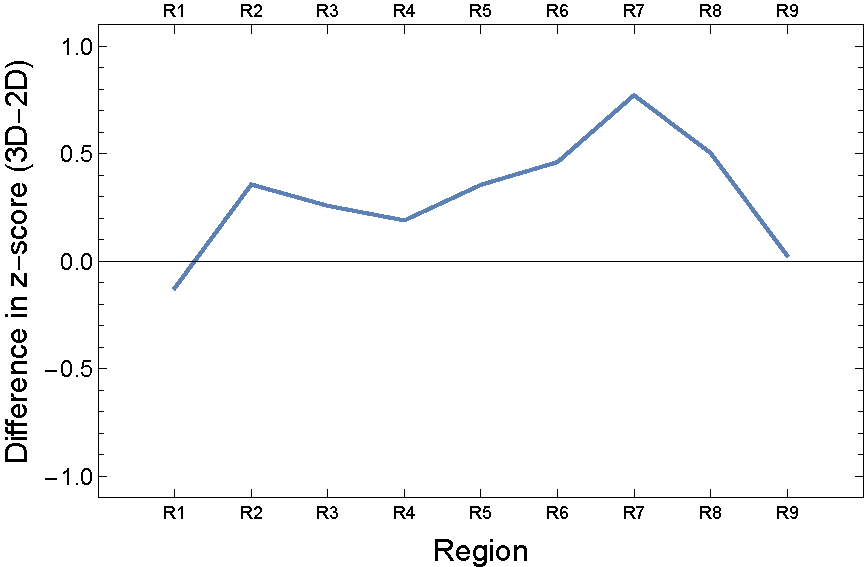
\includegraphics[width=0.8\linewidth]{zScoreByRegion.pdf}
		     \caption{{\color{truetree}Was the bar diagram updated after the bug? }}
		     \label{fig:difference16S}
        \end{figure}

    \begin{table}[h!]
    \centering
    \begin{tabular}{|c|c|c|}
\hline
Region & Z-score 3D tree & Z-score 2D-rearranged tree\\
\hline
R1&4.57&5.08\\
R2&6.12&5.94\\
R3&3.62&3.45\\
R4&6.80&6.83\\
R5&8.99&8.93\\
R6&8.54&8.31\\
R7&8.93&8.35\\
R8&12.44&12.32\\
R9&9.32&9.65\\
\hline
    \end{tabular}
    \vspace{0.25cm}
    \caption{{\color{olive}\textbf{Per-protein z-scores} for the branches leading to Eukaryota in the ML-reconstructed 3D tree (Fig.\,\ref{fig:EUK}c) and the rearranged 2D tree (Supplementary Fig.\,\ref{fig:rRNA_rearranged2Dtree})}}
    \label{tab:rRNA_2D_3D}
    \end{table}

\begin{figure}[H]
            \centering
            \includegraphics[width=0.8\linewidth]{rRNA_based_comparison_2D_3D_diff_zscores.pdf}
		     \caption{{\color{olive}\textbf{Per-protein z-scores comparison to a rearranged topology.} For each protein of the protein alignment, difference in the Satute z-score in the branch leading to Eukaryota between the ML-reconstructed 3D tree (Fig.\,\ref{fig:EUK}c) and the rearranged 2D tree (Supplementary Fig.\,\ref{fig:rRNA_rearranged2Dtree}). }}
		     \label{fig:rRNA_2D_3D}
        \end{figure}

\textbf{Suggestion from Christiane: END}}\\


\begin{figure}[H]
            \includegraphics[width=0.8\linewidth]{indexFigure.pdf}
                       \caption{For the 16S rRNA gene alignment, plots of the z-scores obtained from sliding-window testing ($n=36$) using Satute in the branch leading to Eukaryotes (purple) and the branch-independent saturation index (blue). Grey shadows indicate regions where the branch leading to Eukaryotes is affected by saturation, while the saturation index rejects saturation.}
	\label{fig:indexFigureRNA}
\end{figure}

\begin{figure}[H]
            \includegraphics[width=0.8\linewidth]{indexAA.pdf}
                       \caption{For the ribosomal protein alignment, plots of the z-scores obtained from from sliding-window testing ($n=36$) using Satute in the branch leading to Eukaryotes (purple) and the branch-independent saturation index (blue).}
	\label{fig:indexFigureAA}
\end{figure}

\fi


\end{appendices}